\documentclass{article}
\usepackage{graphicx}
\usepackage{url}
\graphicspath{ {./src/images/} }
\title{Lecture notes of Tor under the hood}
\author{Jaysinh Shukla}
\begin{document}

\maketitle

\section{History}

  The concept of onion routing was developed by the employees of United States
  Naval Research Laboratory employees David Goldschlag, Mike Reed, and Paul
  Syverson. 1997 DARPA further developed the onion routing.
  \cite{history_of_tor} It was the year after when the Internet started getting
  popularity.  It was expected that each country will have the connectivity of
  Internet by 1999 and it became true too.  \cite{digitalrevolution}

  During the year 2000, Roger Dingledine started working further on onion
  routing with Paul Syverson. The project named The Onion Routing (Tor). Since
  1990, the concept of onion routing was developed with a mindset of
  transparency and decentralized network. Because of that, Tor released under
  free and open license.

  In 2006, The Tor project Inc, a Massachusetts based non-profit organization
  was formed to develop and maintain Tor project further. Electronic Frontier
  Foundation(EFF) which is well-known for fighting against privacy and mass
  surveillance found Tor as a potential tool. They started funding Tor then
  U.S.  International Broadcasting Bureau, the University of Cambridge, Google
  and U.S. Government. During the early days, U.S. Government was the major
  source of funding for Tor.

\section{Popularity}

  \subsection{Tor Users}

    \subsubsection{Users of Tor in All around the world}
      \begin{figure}[h!]
        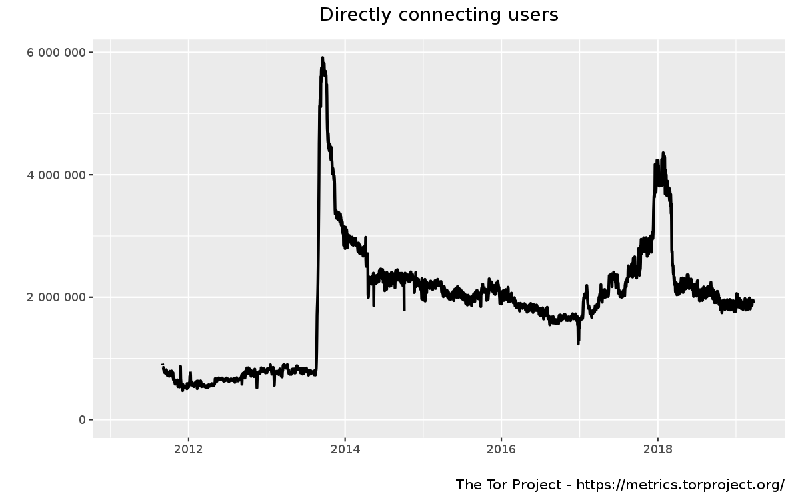
\includegraphics[width=\linewidth]{userstats-relay-country-all-last-decade.png}
        \caption{Users of Tor in last decade. Includes from all around the world}
        \label{fig:users_of_tor_from_all_around_the_world_last_decade}
      \end{figure}

      In last decade, total number of Tor users are doubled. Nearly 1 million
      users were using Tor during the year 2009. The user base has touched to 2
      million post 2014. With some hikes and falls, it is stable to nearly 2
      million active users a day at present. It is to be noted that the graph do
      not include users connecting using bridges. Tor bridges are one way to
      connect through Tor in a region where Tor is banned. I will explain Tor
      bridges at \textbf{Components of Tor} section.


    \subsubsection{Users of Tor in India during last decade}
      \begin{figure}[h!]
        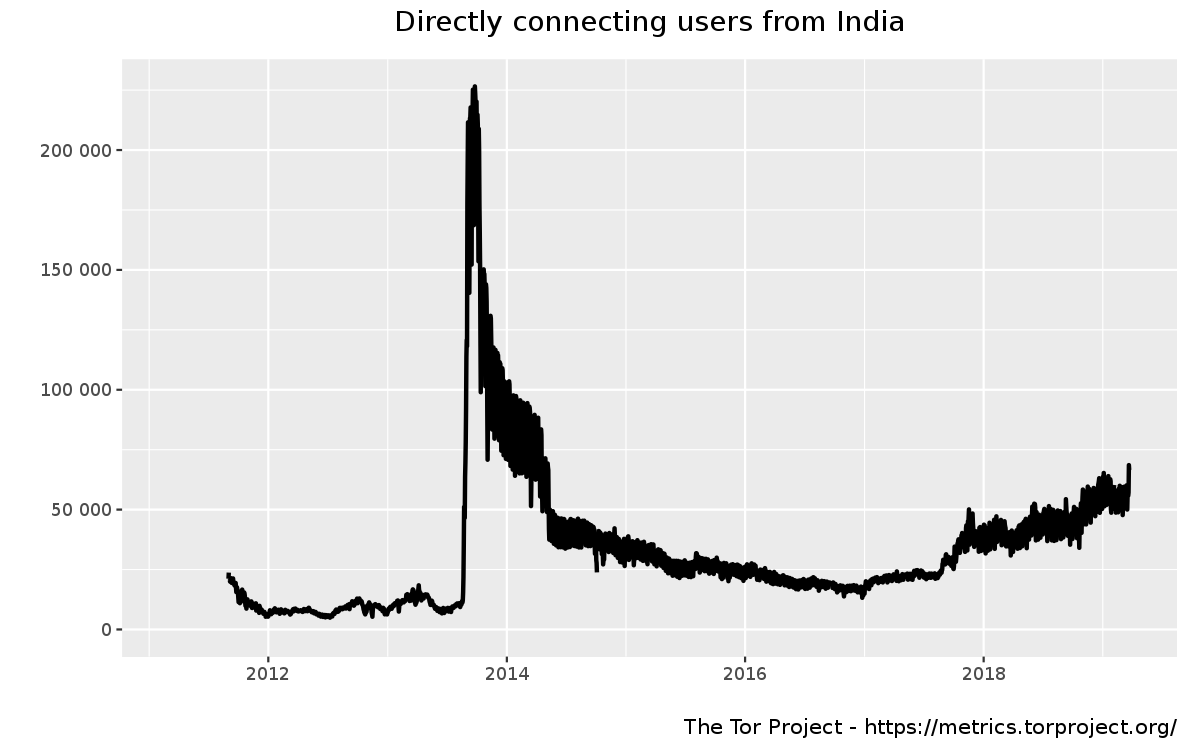
\includegraphics[width=\linewidth]{userstats-relay-country-india-last-decade.png}
        \caption{Users of Tor in last decade. Only from India}
        \label{fig:users_of_tor_from_india_last_decade}
      \end{figure}

      During the year 2009, daily Tor users from India was below 25 thousands.
      The User base doubled post 2014. Then it constantly decreased till half of
      the year 2016. After that it is constantly increasing. At present, it is
      more than 50 thousand daily active users. We can conclude that, Tor users
      of India has been more than doubled during last decade. This records too
      are excluding Users connecting via Tor bridges.

  \subsection{Onion Services}
    \begin{figure}[h!]
      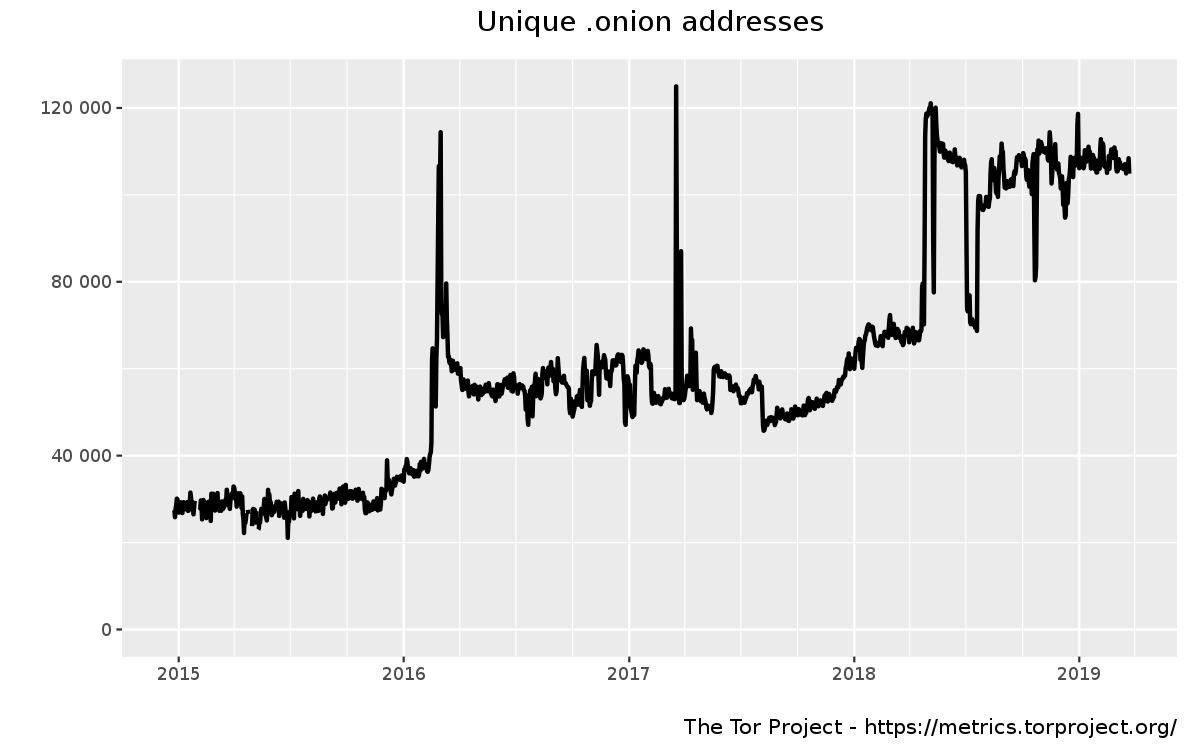
\includegraphics[width=\linewidth]{onion-addresses-in-last-decade.png}
      \caption{Onion services in last decade}
      \label{fig:onion_service_in_last_decade}
    \end{figure}

    Presented graph shows growth of onion addresses. During the year 2015,
    there was more nearly 20 thousand onion addresses. Between the period of a
    half decade or even less than a half decade, the total amount of onion
    addresses are increased 5 times. This clearly depicts the potential of
    onion services. We will learn more about onion addresses at
    \textbf{Components of Tor}

  \subsection{Tor relays}
    \begin{figure}[h!]
      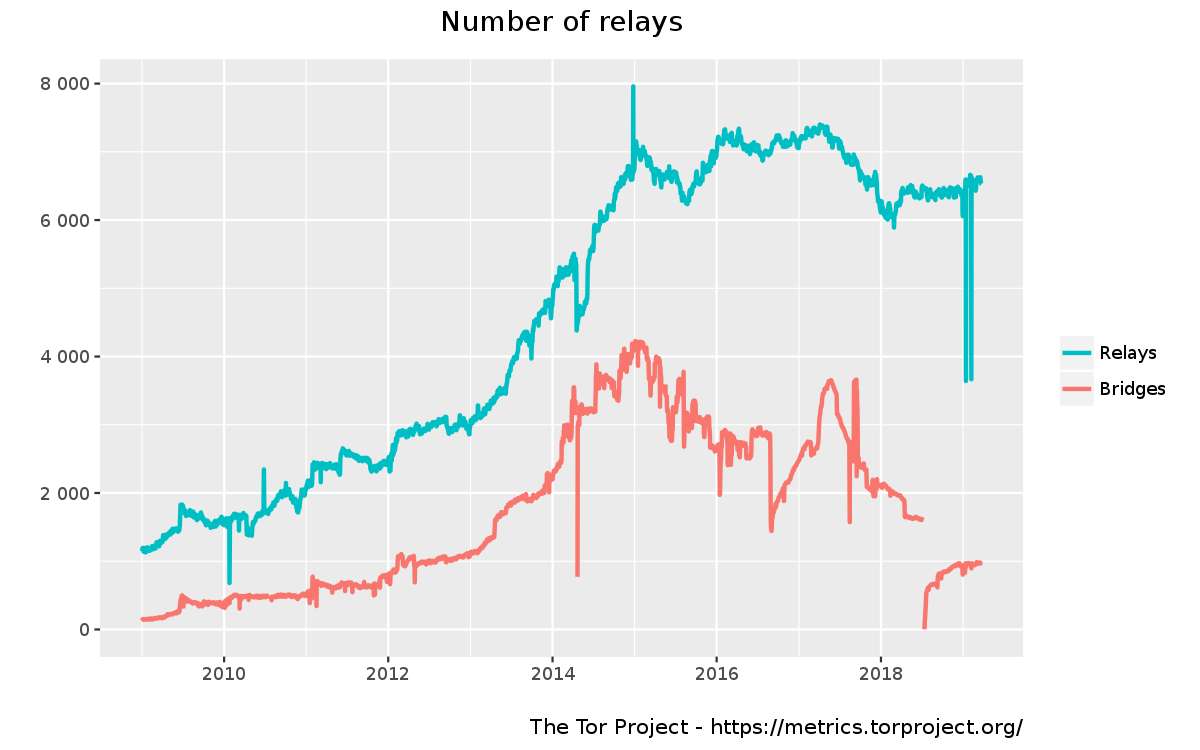
\includegraphics[width=\linewidth]{relays-and-bridges-in-last-decade.png}
      \caption{Tor relays and bridges during last decades}
      \label{fig:relays_and_bridges_during_last_decade}
    \end{figure}

    There were nearly 1 thousand relays were active during the year 2009. The
    relays constantly increased and reached at 8 thousand during the year 2014.
    With few ups and downs, there are more than 6 thousand relays currently.

    I am skipping comparing bridges in this session. I will explain relays and
    bridges at \textbf{Components of Tor} section.

  \section{Components of Tor network}

    \subsection{Tor relays}
      Tor relays are extremely import component of Tor network. Tor relay is a
      piece of software which is run by a volunteer. Job of the Tor relay is to
      route traffic to another relay or to the destination. Tor relay is also
      called a node.

      There are three types of relays

      \begin{itemize}
        \item{Entry node/Guard node}
        \item{Middle node}
        \item{Exit node}
      \end{itemize}

      \subsubsection{Entry node/ Guard node}
        This relay receives request directly from the client. Because it hides
        information of the client from rest of relays in circuit, it is called
        a guard node.

      \subsubsection{Middle node}
        The relay which is at the middle position of the guard node and exit
        node is called a middle node. The middle node is responsible for
        forwarding requests coming from guard node to the exit node. Middle
        node do not know from which source the request is coming.

      \subsubsection{Exit node}
        Exit node is the last node of Tor circuit. Exit node puts It is exit
        node who actually fire the request to the destination. The destination
        website or service will know that the request is coming from the exit
        node, but it doesn't know who has requested. The Exit node don't have
        any information about the Guard node or the source of the request.


      The entry node and middle node do not receive any abusive complains
      because the destination do not know their involvement in routing the
      request. The exit node is susceptible to receive complaints if the end
      request is doing any prohibited things.

      The relays are ran by volunteers. You can be volunteer to run a relay.
      It is comparatively safe to run Guard or Middle node at home. But one
      should not attempt to host exit relay at home. University or public
      network where people can fight with legalities is the best place for exit
      relays.

      Information of the Tor relays are available to public. They are not
      hidden.

    \subsection{Bridge}
      Bridges are the one type of Tor relays which are not listed in to the
      public Tor directory. By doing this, it becomes hard for Government or
      ISP to identify bridge relay. Connecting to Tor network using bridge will
      help in anonymizing that one has connected to Tor network.

      You can run a bridge at your home. Bridges are likely to expect low
      traffic and it doesn't expect high bandwidth.

    \subsection{Tor circuit}
      Circuit is a path on which request will be routed. It includes virtual
      connection of Entry node, Middle node and Exit node. Tor software do not
      use the same circuit to route the package for more than 10 minutes. Such
      sort time is chosen to make tracking user difficult.

      \begin{figure}[h!]
        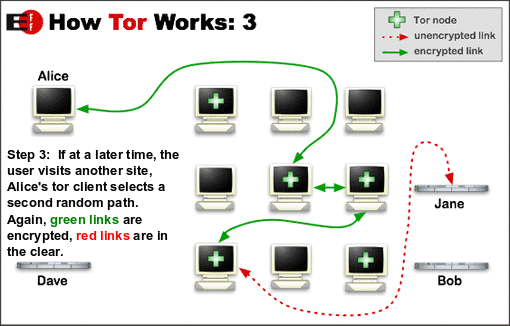
\includegraphics[width=\linewidth]{tor_circuit.png}
        \caption{Tor circuit}
        \label{fig:tor_circuit}
      \end{figure}

      In above diagram, the Request from Alice is transferred to Entry Node and
      then the entry node is forwarding the request to exit node and the Exit
      node is finally reaching the destination Jane. Response from Jane is
      forwarded to Exit node and Exit node forwards the response as it was
      forwarded while requesting.

    \subsection{Onion routing}
      Onion routing is a special technique of routing to anonymize the source
      and destination of the request. Because it includes routing by various
      nested layers hiding details of one layer with the another, like an onion
      it is called an onion routing.

      \begin{figure}[h!]
        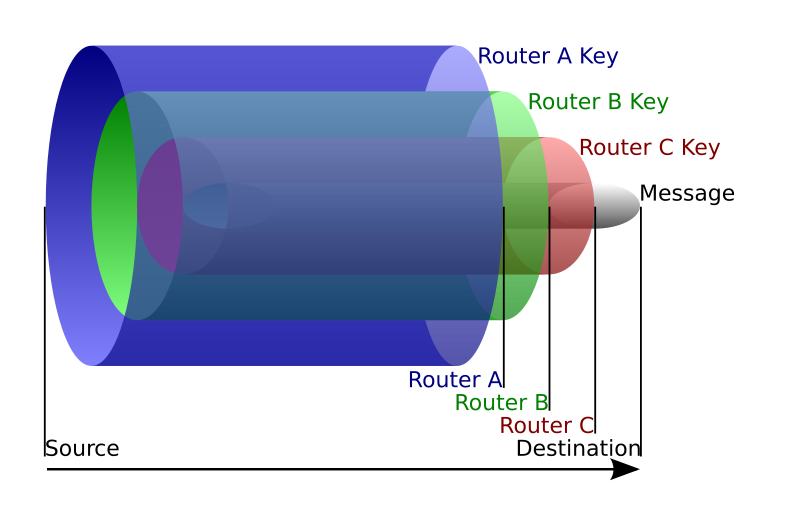
\includegraphics[width=\linewidth]{onion_routing_with_layers.png}
        \caption{Onion routing with layers}
        \label{fig:onion_routing_with_layers}
      \end{figure}

      Let me explain the process from the beginning of the request and how the
      response is forwarded back to the Tor network.

      First the client will generate the Tor circuit. All the node are chosen
      from the publicly available relays directory. The client will generate a
      symmetric key and pass it to the guard node. This key exchange is done
      with public key encryption. The client will generate individual symmetric
      keys for all the relays and pass them to destination relay through Tor
      circuit.

      The request is first wrapped to Exit nodes symmetric key, then with
      symmetric key of the Middle node and then with the symmetric key of the
      entry node. Then the onion packet is transferred to the Entry node. The
      entry node unwraps the packet with its symmetric key and pass the rest of
      the request to the middle node. The middle node unwraps the received
      onion packets and transfer the packet to the Exit node. At the end the
      exit node unwraps the onion packet and finds the destination to where it
      has to fire the request. The exit node fires request and receives the
      response from the destination. The exit node wraps the response with its
      symmetric key and pass it to the middle node. The same wrapping process
      is followed by guard and middle node and the onion packet is received to
      the source. The source unwraps all three layers and finds the response.

      The process of wrapping and constructing onion packet is repeated for
      every request. Involved relays are changed every 10 minutes and new
      symmetric keys are generated and exchanged with new relays to increase
      the security.

    \section{Comparison of browsing through Tor and HTTPS}

      \begin{figure}[h!]
        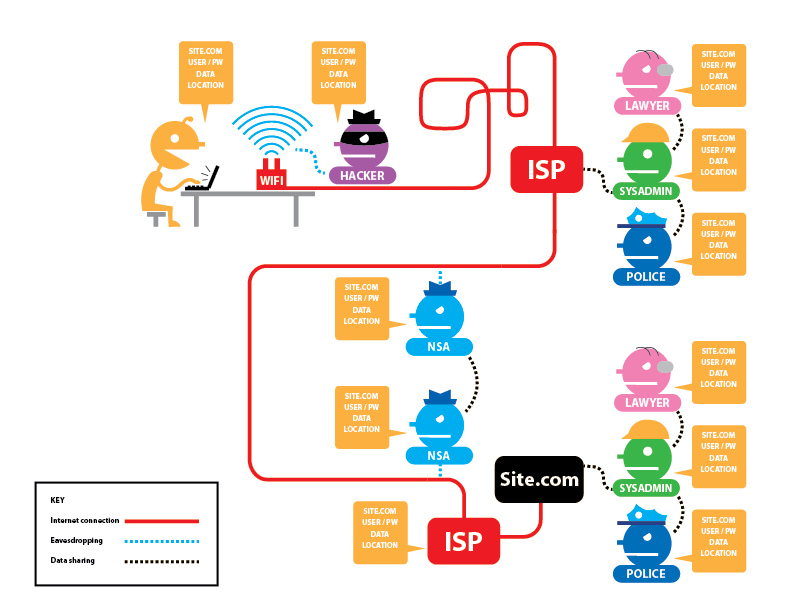
\includegraphics[width=\linewidth]{no_tor_no_https.png}
        \caption{Information one expose when browsing without Tor and HTTPS}
        \label{fig:no_https_no_tor}
      \end{figure}

      When browsing without Tor or HTTPS, information like which website are
      you browsing and formdata and Submitted Username and Password are exposed
      when the request is routing to its destination.

      \begin{figure}[h!]
        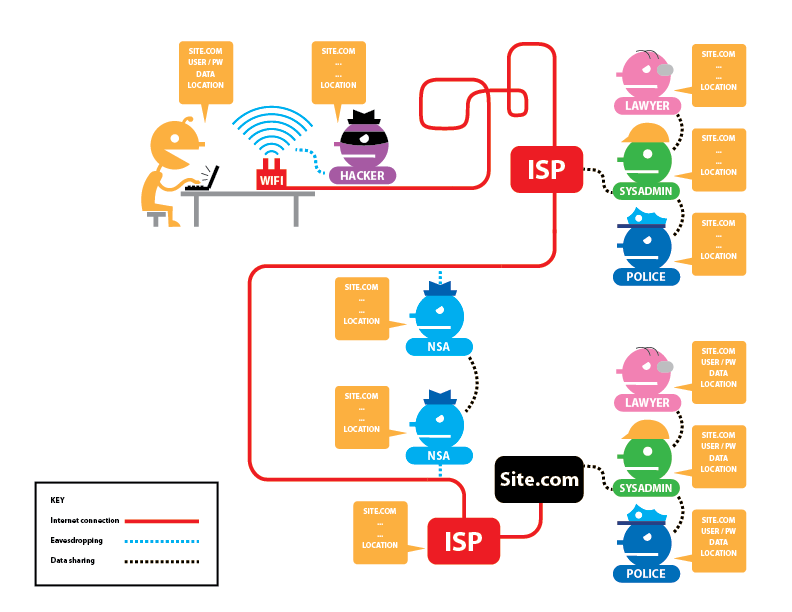
\includegraphics[width=\linewidth]{no_tor_yes_https.png}
        \caption{Information one expose when browsing without Tor but with HTTPS}
        \label{fig:no_https_no_tor}
      \end{figure}

      When HTTPS is used for communicating with destination, lot of information
      is hidden. The request does hides formdata and sensitive information like
      Username and password from the middle eavesdroppers. But they are still
      able to identify the location of the source because it is exposing the IP
      address and location of destination website. Even if source is using
      HTTPS, it is possible to track which website the user is visiting and who
      is that user.

      \begin{figure}[h!]
        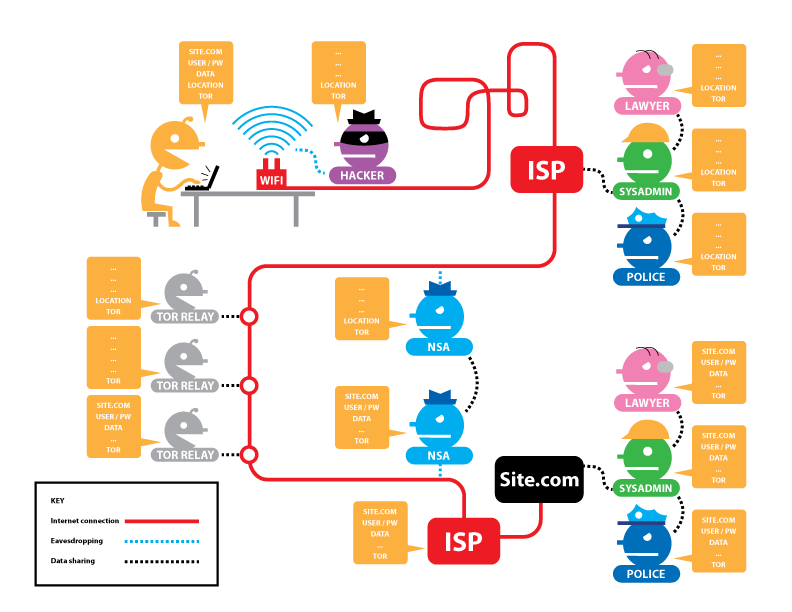
\includegraphics[width=\linewidth]{yes_tor_no_https.png}
        \caption{Information one expose when browsing with Tor but without HTTPS}
        \label{fig:no_https_no_tor}
      \end{figure}

      When Tor is used to surf without using HTTPS, It hides information like
      Username and password from the man in the middle, but the exit node
      exposes them while putting request. Tor does expose location of the User
      until the request reaches first hope, but it hides information like what
      site the user wants to visit. It is to be noted that people can identify
      that you are using Tor. Tor traffic looks similar when transiting in the
      network.


      \begin{figure}[h!]
        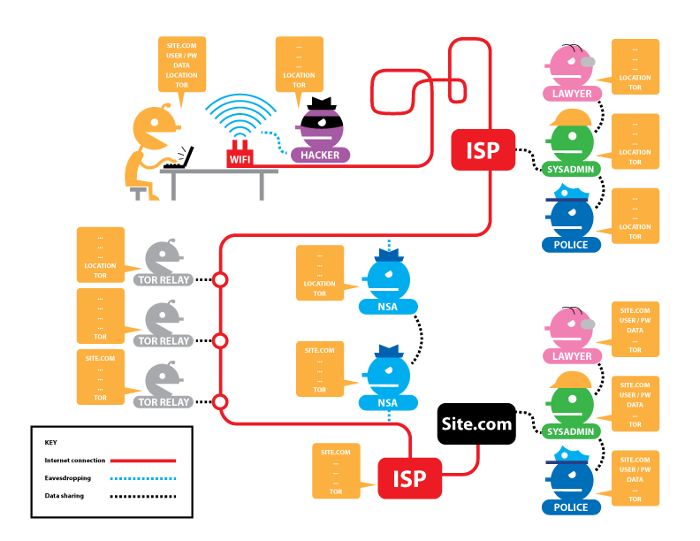
\includegraphics[width=\linewidth]{yes_tor_yes_https.png}
        \caption{Information one expose when browsing with Tor and HTTPS}
        \label{fig:no_https_no_tor}
      \end{figure}

      When Tor is used with HTTPS, it provides great level of security. It
      hides information like Username and password and other body information
      when the exit node resolves the request. As I have mentioned, Location
      details of the User is exposed until the request reaches first relay.
      Though it hides information like which site the user is trying to browse.

      \begin{figure}[h!]
        
\includegraphics[width=\linewidth]{incognito_mode.png}
        \caption{Information exposed when browsing through incognito mode}
        \label{fig:incognito_mode}
      \end{figure}

      Browsing through incognito doesn't hide anything from people involved at
      network level, eavesdroppers, NSA or anyone listening your traffic. It
      exposes your IP information, information like your operating system,
      browser details, which website you are trying to observe etc.

\begin{thebibliography}{2}

  \bibitem{digitalrevolution}
    Wikipedia Digital Revolution
    \url{https://en.wikipedia.org/wiki/Digital_Revolution#1990s}

  \bibitem{history_of_tor}
    History of Tor
    \url{https://www.torproject.org/about/history/}

\end{thebibliography}

\end{document}
